%%%%%%%%%%%%%%%%%%%%%%%%%%%%%%%%%%%%%%%%%
% Beamer Presentation
% LaTeX Template
% Version 1.0 (10/11/12)
%
% This template has been downloaded from:
% http://www.LaTeXTemplates.com
%
% License:
% CC BY-NC-SA 3.0 (http://creativecommons.org/licenses/by-nc-sa/3.0/)
%
%%%%%%%%%%%%%%%%%%%%%%%%%%%%%%%%%%%%%%%%%

%----------------------------------------------------------------------------------------
%	PACKAGES AND THEMES
%----------------------------------------------------------------------------------------

\documentclass{beamer}

\mode<presentation> {
\usepackage[utf8]{inputenc} %unicode support
% The Beamer class comes with a number of default slide themes
% which change the colors and layouts of slides. Below this is a list
% of all the themes, uncomment each in turn to see what they look like.

%\usetheme{default}
%\usetheme{AnnArbor}
%\usetheme{Antibes}
%\usetheme{Bergen}
%\usetheme{Berkeley}
%\usetheme{Berlin}
%\usetheme{Boadilla}
%\usetheme{CambridgeUS}
%\usetheme{Copenhagen}
%\usetheme{Darmstadt}
%\usetheme{Dresden}
%\usetheme{Frankfurt}
%\usetheme{Goettingen}
%\usetheme{Hannover}
%\usetheme{Ilmenau}
%\usetheme{JuanLesPins}
%\usetheme{Luebeck}
\usetheme{Madrid}
%\usetheme{Malmoe}
%\usetheme{Marburg}
%\usetheme{Montpellier}
%\usetheme{PaloAlto}
%\usetheme{Pittsburgh}
%\usetheme{Rochester}
%\usetheme{Singapore}
%\usetheme{Szeged}
%\usetheme{Warsaw}

% As well as themes, the Beamer class has a number of color themes
% for any slide theme. Uncomment each of these in turn to see how it
% changes the colors of your current slide theme.

%\usecolortheme{albatross}
%\usecolortheme{beaver}
%\usecolortheme{beetle}
%\usecolortheme{crane}
%\usecolortheme{dolphin}
%\usecolortheme{dove}
%\usecolortheme{fly}
%\usecolortheme{lily}
%\usecolortheme{orchid}
%\usecolortheme{rose}
%\usecolortheme{seagull}
%\usecolortheme{seahorse}
%\usecolortheme{whale}
%\usecolortheme{wolverine}

%\setbeamertemplate{footline} % To remove the footer line in all slides uncomment this line
%\setbeamertemplate{footline}[page number] % To replace the footer line in all slides with a simple slide count uncomment this line

%\setbeamertemplate{navigation symbols}{} % To remove the navigation symbols from the bottom of all slides uncomment this line
}

\usepackage{graphicx} % Allows including images
\usepackage{booktabs} % Allows the use of \toprule, \midrule and \bottomrule in tables

%----------------------------------------------------------------------------------------
%	TITLE PAGE
%----------------------------------------------------------------------------------------

\title[Alignment-free tools]{Alignment-free tools for metagenomics-data analysis } % The short title appears at the bottom of every slide, the full title is only on the title page

\author{Robert Deibel} % Your name
\institute[Universität Tübingen] % Your institution as it will appear on the bottom of every slide, may be shorthand to save space
{
Eberhard-Karls Universität Tübingen \\ % Your institution for the title page
\medskip
\textit{robert.deibel@student.uni-tuebingen.de} % Your email address
}
\date{\today} % Date, can be changed to a custom date

\begin{document}

\begin{frame}
\titlepage % Print the title page as the first slide
\end{frame}

\begin{frame}
\frametitle{Overview} % Table of contents slide, comment this block out to remove it
\tableofcontents % Throughout your presentation, if you choose to use \section{} and \subsection{} commands, these will automatically be printed on this slide as an overview of your presentation
\end{frame}

%----------------------------------------------------------------------------------------
%	PRESENTATION SLIDES
%----------------------------------------------------------------------------------------

%------------------------------------------------
\section{Metagenomics} % Sections can be created in order to organize your presentation into discrete blocks, all sections and subsections are automatically printed in the table of contents as an overview of the talk
%------------------------------------------------

\begin{frame}
\frametitle{Metagenomics}
\subsection{Metagenome}
\begin{block}{Metagenome}
                            \begin{itemize}
               	\item  A metagenome is the whole set of transcripts found in a sample.
                        \item Metagenomics is the study of those
                        \item $>90\%$ uncultureable microorganisms
                        \item design of antibiotics, analysis of microorganismal life    
                        \end{itemize}
\end{block}
\subsection{NGS and alignment}
\begin{block}{NGS and alignment}
\begin{itemize}
\item Advances in sequencing made metagenomics possible
\item NGS generates comparable reads
\end{itemize}
\end{block}
\end{frame}

%------------------------------------------------
\begin{frame}
\frametitle{Metagenomics}
	\begin{block}{Goals}
		\begin{itemize}
			\item insight in microorganismal life
			\item first evidence of origin and function
			\item independent from databases and coding regions
		\end{itemize}
	\end{block}
\end{frame}

%------------------------------------------------
\section{Alignment-based approach}
\begin{frame}
	\frametitle{Alignment-based approach}
	\uncover<1,2>{\begin{block}{Advantages}
		\begin{itemize}
			\item Align sequences against database
			\item Profiles can be analyzed
			\item BLAST $>80\%$ accuracy
		\end{itemize}
	\end{block}}
\uncover<2>{\begin{block}{Disadvantages}
	\begin{itemize}
		\item Low speed
		\item Dependent of databases
		\item Unsequenced transcripts cannot be matched
		\item Databases mostly consist of coding sequences
	\end{itemize}
\end{block}}
	
\end{frame}
%-----------------------------------------------
\section{Alignment-free methods}
\begin{frame}
\frametitle{Different approaches}
	\begin{block}{Statistics}
		\begin{itemize}
			\item Utilizes statistics differing in power
			\item based on $k$-tuple counts
			\item Have to be applied through (dis)similarity matrix
			\item Further analysis follows
		\end{itemize}
	\end{block}
\begin{block}{Machine learning}	
	\begin{itemize}
		\item Optimization of a function
		\item based on $k$-mer signature
		\item applies BH-SNE
		\item Visualizes data in scatter plots
	\end{itemize}
\end{block}
\end{frame}

%------------------------------------------------
\subsection{Statistics as similarity measurement}
\begin{frame}
	\frametitle{Measuring similarity}
	$$D_2=\sum_{w\in \mathcal{A}^k}X_wY_w$$
	where:
	\begin{itemize}
		\item $X_w$, $Y_w$ number of occurrences in $A$, $B$
		\item $\mathcal{A}$ alphabet
		\item $k$ is length of $w$
	\end{itemize}
\uncover<2>{\begin{block}{Problem}
		$D_2$ is not normalized $\Rightarrow$ results vary on different factors
\end{block}}
\end{frame}

%-----------------------------------------------

\begin{frame}
	\frametitle{Measuring similarity}
		Assume sequences are generated through Markov chain\\
		\uncover<2,3,4,5>{$$D2z(A,B)=\frac{D_2(A,B)-E(D_2)}{\sqrt{Var(D_2)}}$$}%
		\begin{itemize}
		\uncover<3,4,5>{\item compared to five other measures $D2z$ outperformed them}\\
		\uncover<4,5>{\item needs two parameters, $k$ and $r$}
		\uncover<5>{\item $E(D_2)$ and $Var(D_2)$ calculated with Markov chain in mind}
	\end{itemize}
\end{frame}

%-----------------------------------------------

\begin{frame}
	\frametitle{Calculating the expected value}
	\begin{block}{MC of order zero}
		Probability of $A=B$ or\dots\\
		\uncover<2,3,4,5>{Sum of background probabilities $f_a^A$, $f_a^B$ to the power of $k$}
		\uncover<3,4,5>{$$E(D_2)=\left(\sum_{a\in \mathcal{A}}f_a^Af_a^B\right)^k$$}
	\end{block}
\uncover<4,5>{\begin{block}{MC of order 1}
	Sum of probabilities for $|w|=k$, under consideration of MC\\
	\uncover<5>{$$\sum_{|w|=k}p^A(w_1)p^A(w|w_1)p^B(w_1)p^B(w|w_1)$$}
\end{block}}
\end{frame}


%------------------------------------------------

\subsection{CVTree}
\begin{frame}
\frametitle{Constructing phylogenetic trees -- CVTree}
	\begin{itemize}
		\item considers (k-2)-th order MC estimated by $E^X_w$
		\uncover<2,3,4>{$$Hao=\frac{1}{2}(1-C)$$}
		\uncover<3,4>{$$C=\frac{\sum_w\left(\frac{X_w-E_w^X}{E_w^X}\right)\left(\frac{Y_w-E_w^Y}{E_w^Y}\right)}{\sqrt{\sum_w\left(\frac{X_w-E_w^X}{E_w^X}\right)^2\sum_w\left(\frac{Y_w-E_w^Y}{E_w^Y}\right)^2}}$$}
		\uncover<4>{\item Observations in composition vector
		\item subtraction of background "noise" through MC
		\item $C$ is cosine between vectors}
	\end{itemize}
\end{frame}

\begin{frame}\begin{figure}
		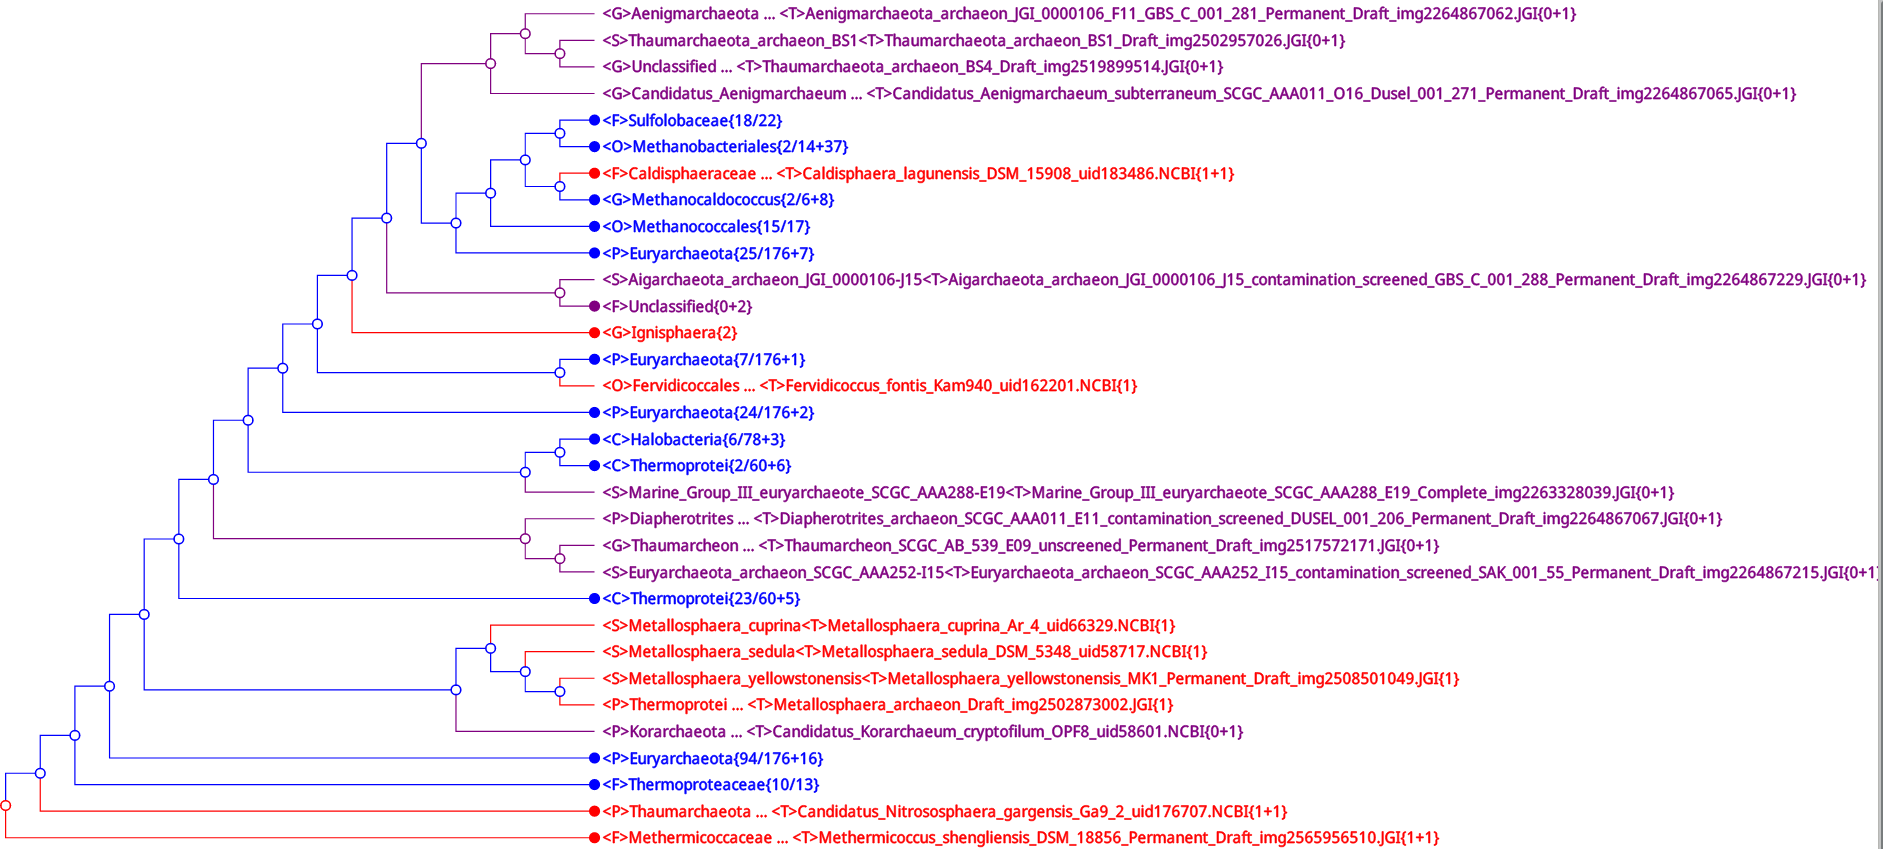
\includegraphics[width=\linewidth]{bilder/CVTree.png}
	\caption{Computed phylogenetic tree through application of neighbor joining dissimilarity matrix}
\end{figure}
\end{frame}
%--------------------------------------------------

\begin{frame}
	\frametitle{Nucleotide frequency}
	\begin{itemize}
		\item Related approach to $Hao$
		\item Consider di-nucleotide frequency
		$$\rho_{ab}(A)=\frac{f_{ab}}{f_af_b}$$
		\item Can be extended to tri- and tetra nucleotides
		\item $l_p$ norm as dissimilarity measure
		$$\delta(A,B)=\sum_{ab\in A}|\rho_{ab}(A)-\rho_{ab}(B)|$$
	\end{itemize}
\end{frame}

%------------------------------------------------
\subsection{$D_2^S$, $D_2^*$ and their normalization}
\begin{frame}
	\frametitle{$D_2^S$, $D_2^*$ and their normalization}
	\begin{itemize}
		\item For two normal random variables $XY/\sqrt{X^2+Y^2}$ is also normally distributed
		\uncover<2,3,4>{$$D_2^S=\sum_{w\in \mathcal{A}^k}\frac{\widetilde{X}_w\widetilde{Y}_w}{\sqrt{\widetilde{X}_w^2+\widetilde{Y}_w^2}}$$}%
		\uncover<3,4>{\item$D_2^*$ utilizes that number of occurrences is approximately Poisson; mean and variance are the same}
		\uncover<4>{\begin{block}{Conclusions}
				\begin{enumerate}
					\item $D_2^S$ and $D_2^*$ have higher power than $D_2$
					\item $D_2^*$ has highest power when $k$ equals $motif$ length
					\item $D_2^*$ has higher power for short sequences\\
			
				\end{enumerate}
				but again both not normalized
	\end{block}}
		
	\end{itemize}
\end{frame}

%------------------------------------------------
\begin{frame}
\frametitle{Normalization and Neighborhood}
\begin{block}{Normalization}
	\begin{itemize}
		\item Normalization to $d_2^S$ and $d_2^*$
		\item 0 when sequences are the same and close to one if anti-correlated
		\item Now applicable to metagenomic data or varying types of sequences
	\end{itemize}
\end{block}
%-----------------------------------------------
\subsection{Consideration of mismatches}
\uncover<2>{\begin{block}{Consideration of mismatches}
	\begin{itemize}
		\item instead of $w$ the statistics should consider the neighborhood $\varsigma(w)$
		\item If $w' \in \varsigma(w)$ $w'$ has a certain number of mismatches with $w$
		\item Reverse complement can be included similarly
		\item statistics can then be modified
	\end{itemize}
\end{block}}
\end{frame}

%-----------------------------------

\begin{frame}
	\frametitle{Performance under the mismatch model}
	\begin{block}{Test parameters}
		\begin{itemize}
			\item sequences from mouse embryo
			\item positive and negative set maximum of 30\% repetitions
			\item Dissimilarity was calculated
			\item Threshold was applied
			\item  prediction of dissimilarity lower than threshold resulted in positives
			\item Predictions were compared to real data
			\item Testing with different parameters for $k$, $r$ and mismatch weight
		\end{itemize}
	\end{block}
\uncover<2>{\begin{block}{Test conclusions}
	\begin{itemize}
		\item $Hao$ performed worse than $d_2^S$ and $d_2^*$
		\item $d_2^S$ and $d_2^*$ performed best with mismatch weight of 0.05 and $k=4$
		\item Overall $d_2^S$ achieved best results in testing 
	\end{itemize}
\end{block}}
\end{frame}

\subsection{Machine learning -- BH-SNE}

\begin{frame}
	\frametitle{Machine learning -- BH-SNE}
	\begin{itemize}
		\item Applies Barnes-hut and vantage point trees
		\item Utilizes species-specific oligonucleotide signatures as $k$-mers
		\item $k$-mers are represented as vectors in high-dimensional Euclidean space
		\item Transformation enables human interpretation in scatter plots
	\end{itemize}
\end{frame}

%------------------------------------------------

\begin{frame}[fragile] % Need to use the fragile option when verbatim is used in the slide
\frametitle{Citation}
An example of the \verb|\cite| command to cite within the presentation:\\~

This statement requires citation \cite{p1}.
\end{frame}

%------------------------------------------------

\begin{frame}
\frametitle{References}
\footnotesize{
\begin{thebibliography}{99} % Beamer does not support BibTeX so references must be inserted manually as below
\bibitem[Smith, 2012]{p1} John Smith (2012)
\newblock Title of the publication
\newblock \emph{Journal Name} 12(3), 45 -- 678.
\end{thebibliography}
}
\end{frame}

%------------------------------------------------

\begin{frame}
\Huge{\centerline{The End}}
\end{frame}

%----------------------------------------------------------------------------------------

\end{document}